\section{A finite cycle with mean frequency below the degree}
\label{n:sec-angular-program}

The adjacent doubles of Lemma~\ref{n:lem-adjacent-doubles} supply the
individual exchanges. We join them into a closed path and average the
frequencies visited by its continued eigenlines. The finite program is
fixed before its radial starting time and crossing controls are chosen.

A label will now follow a smooth eigenline through each double.  It is
not renamed by its increasing spectral position after a crossing.
Figure~\ref{fig:ang-crossing-cycle} illustrates this continuation and
the adjacent-swap order.
\begin{figure}[tbp]
\centering
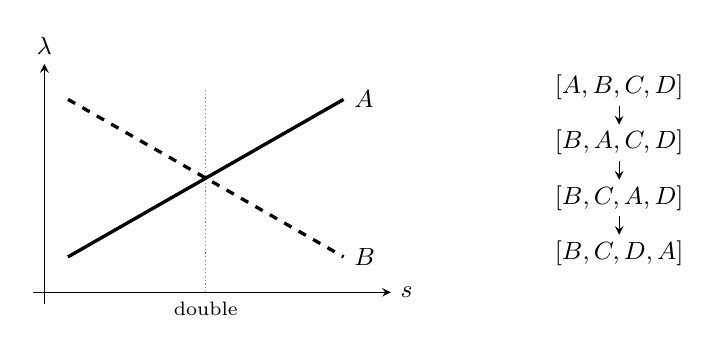
\begin{tikzpicture}[x=1cm,y=1cm,>=stealth,font=\small]
  \draw[->] (0,0.15) -- (4.55,0.15) node[right] {$s$};
  \draw[->] (0.15,0) -- (0.15,3.05) node[above] {$\lambda$};
  \draw[gray,densely dotted] (2.2,0.15) -- (2.2,2.75);
  \draw[very thick] (0.45,0.6) -- (3.95,2.6) node[right] {$A$};
  \draw[very thick,dashed] (0.45,2.6) -- (3.95,0.6) node[right] {$B$};
  \node[font=\scriptsize,below] at (2.2,0.15) {double};

  \node at (7.45,2.75) {$[A,B,C,D]$};
  \node at (7.45,2.05) {$[B,A,C,D]$};
  \node at (7.45,1.35) {$[B,C,A,D]$};
  \node at (7.45,0.65) {$[B,C,D,A]$};
  \draw[->] (7.45,2.52) -- (7.45,2.28);
  \draw[->] (7.45,1.82) -- (7.45,1.58);
  \draw[->] (7.45,1.12) -- (7.45,0.88);
\end{tikzpicture}
\caption{Schematic of a continued pair at an isolated double (left)
and the increasing adjacent-swap schedule on four illustrative ranks
(right). The solid line $A$ changes from lower to upper ordered rank;
the four-rank schedule sends the first label to the last rank. No
numerical eigenvalues or phase durations are represented.}
\label{fig:ang-crossing-cycle}
\end{figure}

In the statement below, \(\lambda_j(H(s))\) still means the ordered
eigenvalue of the metric, while \(\lambda_i(s)\) means the eigenvalue
of the continued line with initial label \(i\).

\begin{proposition}[Angular program]\label{n:prop-angular-program}
Fix \(2/3<a<1\), \(1<\vartheta<3a/2\), and
\(a^2<\kappa_*<1\).  Prescribe a sufficiently small conformal
neighborhood \(\mathcal U\) for which the curvature and comparison
bounds above hold.  For every sufficiently large integer \(k\), with
threshold allowed to depend on \(\mathcal U\),
there are \(S>0\) and a smooth \(S\)-periodic path \(w(s)\) in
\(\mathcal U\) such that \(H(s)=h(w(s))\) has the following
properties, with \(M,p,L,I,N\) as in \eqref{n:eq-band}.
The phase origin can be chosen so that \(w(s)=w(0)\) for
\(|s|<\varepsilon_0\), for some \(\varepsilon_0>0\), and
\(h(w(0))\) is simple through position \(p+1\).
\begin{enumerate}
\item The area form is \(d\operatorname{vol}_{H(s)}=4\pi\,d\mu\)
      pointwise, and the ordered outer gap
      \(\lambda_p(H(s))<\lambda_{p+1}(H(s))\) holds for every \(s\).
\item Along the unwrapped path \(s\in\mathbb R\), the spectral subspace
      of the first \(p\) positions has a smooth real
      \(L^2(d\mu)\)-orthonormal frame
      \(e_1(s),\ldots,e_p(s)\) of continued eigenlines.  Their
      only equalities are isolated double crossings at distinct
      phases, and at each crossing the traceless first derivative
      of its \(2\times2\) cluster matrix is nonzero.  The return
      permutation after \(S\) fixes positions \(1,\ldots,B_L\)
      and is one cycle on \(I\).
\item With
      \[
       d(x)=\frac{-1+\sqrt{1+4x}}2,
      \]
      every label among the first \(p\) satisfies
      \begin{equation}\label{n:eq-frequency-margin}
       \frac1{NS}\int_0^{NS}d\bigl(a^{-2}\lambda_i(s)\bigr)\,ds<k.
      \end{equation}
      Here \(NS\) is an eigenvalue period for every band label and
      also a period for every fixed lower label.
\end{enumerate}
At each crossing there is a smooth conformal direction \(\xi\) for
which the off-diagonal entry
\[
 \left\langle e_h,
     \left.\frac{d}{d\varepsilon}\right|_{\varepsilon=0}
        (-\Delta_{h(w+\varepsilon\xi)})e_i
 \right\rangle_{L^2(d\mu)}
\]
is nonzero on the crossing pair.  After \(k\) and the entire program
are fixed, the outer gap, the absolute crossing slopes, and the
separations between crossing phases have positive uniform lower
bounds.  For every fixed order, the smooth norms of the frame and
metrics have a uniform upper bound.  For each pair, its absolute
eigenvalue gap has a positive lower bound on every compact subset of
the full label-period phase circle \(\mathbb R/(NS\mathbb Z)\)
disjoint from that pair's crossing set.  A pair with no crossings
has a uniform gap on that whole circle.
\end{proposition}

\begin{proof}
Before choosing \(k\), shrink the prescribed convex neighborhood
\(\mathcal U\) if necessary so that the mass-form min--max comparison
gives, for every \(w\in\mathcal U\),
\begin{equation}\label{n:eq-near-round-frequency-bound}
 \lambda_j(h(w))\leq C_*\,l(l+1)
 \quad\text{when }B_{l-1}<j\leq B_l,
 \qquad \frac{2\vartheta}{3a}\sqrt{C_*}<1 .
\end{equation}
This is possible because \(C_*\) tends to \(1\) as the neighborhood
shrinks and \(\vartheta<3a/2\).  Lemma~\ref{n:lem-adjacent-doubles}
applies in this smaller neighborhood for every sufficiently large \(k\).

At each double from Lemma~\ref{n:lem-adjacent-doubles}, choose a
conformal direction for which the traceless first derivative of the
two-dimensional cluster matrix is nonzero.  On a short path
through the double, write its matrix as \(M(\tau)\), with
\(M(0)=\lambda I\).  The trace-free quotient
\[
 \widehat M(\tau)=
 \frac{M(\tau)-\tfrac12\operatorname{tr}M(\tau)I}{\tau}
 \quad(\tau\ne0)
\]
extends smoothly across zero.  Its value there is a nonzero
trace-free symmetric \(2\times2\) matrix and therefore has two
distinct eigenvalues.  Its two eigenlines extend smoothly for
small positive and negative \(\tau\).  They are also the
eigenlines of \(M(\tau)\), whose corresponding eigenvalues have
the form
\[
 \tfrac12\operatorname{tr}M(\tau)+\tau\nu_+(\tau),
 \qquad
 \tfrac12\operatorname{tr}M(\tau)+\tau\nu_-(\tau),
 \qquad \nu_+(0)>\nu_-(0).
\]
Their increasing order reverses at zero.  Thus the continued lines
exchange exactly the designated adjacent positions and their
eigenvalue difference has a simple zero.  This is the nonzero
first-order splitting meant here: the path is deliberately chosen
through the codimension-two double condition.

Choose one base parameter simple through \(p+1\).  The endpoints
of each short crossing segment are also simple through \(p+1\);
by Lemma~\ref{n:lem-avoidance}, join each of them to the base by
simple paths in \(\mathcal U\).  The resulting loop has only its
designated double through position \(p+1\).  Smoothly reparametrize
the pieces so they are constant near their joins and near the
base, while retaining nonzero speed at the crossing.  Since the
designated pair lies inside \(I\), every one of these loops keeps
the gap between positions \(p\) and \(p+1\).

Concatenate the loops in the order
\[
 i=B_L+1,\ B_L+2,\ \ldots,\ p-1
\]
and smooth them at their constant base intervals.  If \(C\) denotes
the return permutation of labels on the band, this order gives
\begin{equation}\label{n:eq-return-cycle}
 C(B_L+1)=p,\qquad C(j)=j-1\quad(B_L+2\leq j\leq p).
\end{equation}
It is a single \(N\)-cycle, and positions \(1,\ldots,B_L\) are
fixed.  Extend the resulting parameter loop periodically with period
\(S\), choosing the phase origin inside one of the constant base
intervals.  Its fixed-area image \(H(s)\) is periodic because the gauge
depends only on the current parameter.

Simple eigenlines extend smoothly on the simple portions of the path,
and the quotient construction above extends the two lines at every
double.  We may consequently choose a smooth orthonormal real
eigenframe on the unwrapped line, with \(e_1=1\).  After \(N\)
periods each band line returns to its original line.  Real unit
sections can acquire signs, which can be continued consistently;
after at most \(2NS\) the chosen frame repeats.  These signs change
neither the ordered positions nor the eigenvalues.  There are only
finitely many crossing types in a label period.  Compactness and
the strict properties of the constructed loops give the asserted
uniform outer gap, crossing slopes, phase separations, and smooth
bounds.  The same compactness gives a positive gap for each pair on
every compact subset of the full label-period phase circle disjoint
from that pair's crossing set.

For clarity, every pair of band labels does cross during a label
period.  In one basic period the label entering at position \(B_L+1\)
successively crosses the other \(N-1\) labels and ends at \(p\).
By \eqref{n:eq-return-cycle}, every label takes that entering
position in one of the \(N\) repetitions.  Lower labels never
cross.  At any of these doubles, Lemma~\ref{n:lem-two-directions}
lets us prescribe a nonzero off-diagonal traceless entry in the
continued two-line frame.  Its value in the fixed-area gauge is
unchanged, which supplies the stated direction.  The finite
phase separation allows these directions to be localized near
individual crossings in the later radial construction.

It remains to estimate the frequencies.  The function \(d\)
is the nonnegative solution of \(d(d+1)=x\), so \(d(x)\leq\sqrt x\).
At every ordered position of the round degree-\(l\) block,
\eqref{n:eq-near-round-frequency-bound} yields
\[
 d\bigl(a^{-2}\lambda_j(H(s))\bigr)
 <a^{-1}\sqrt{C_*}\,(l+1).
\]
A label fixed among the first \(B_L\) ranks therefore has frequency
at most \(a^{-1}\sqrt{C_*}\,(L+1)=O(\sqrt{k})<k\) for all
sufficiently large \(k\).

Now fix a band label \(i\).  At a noncrossing phase \(t\in[0,S]\),
let \(\sigma_t\) send a label's rank at the base to its ordered
rank at that phase of the first period.  In the \(n\)-th repetition,
the rank of label \(i\) at that phase is
\(\sigma_t C^n(i)\).  As \(0\leq n<N\), these ranks run once
through \(I\).  Crossing phases form a finite set and do not affect
the integral.  Therefore
\begin{align}
 \frac1{NS}\int_0^{NS}d\bigl(a^{-2}\lambda_i(s)\bigr)\,ds
 &=\frac1{NS}\int_0^S
       \sum_{j\in I}d\bigl(a^{-2}\lambda_j(H(t))\bigr)\,dt
       \notag\\
 &\leq a^{-1}\sqrt{C_*}\,
   \frac{\displaystyle\sum_{l=L+1}^{M}(2l+1)(l+1)}
        {\displaystyle(M+1)^2-(L+1)^2}.
 \label{n:eq-band-frequency-average}
\end{align}
This identity explains why the durations allotted to the individual
loops impose no further condition: at each phase the label samples
every band rank over the \(N\) repetitions.

Since \(L/k\to0\) and \(M/k\to\vartheta\), the ratio of the sum to
the denominator in \eqref{n:eq-band-frequency-average}, divided by
\(k\), tends to \(2\vartheta/3\).  More explicitly, the numerator is
\[
 \sum_{t=L+2}^{M+1}(2t^2-t)
 =\frac23\bigl((M+1)^3-(L+1)^3\bigr)+O(M^2+L^2),
\]
and the denominator is \((M+1)^2-(L+1)^2\).  By
\eqref{n:eq-near-round-frequency-bound}, the limiting bound after
division by \(k\) is \(2\vartheta\sqrt{C_*}/(3a)<1\).
Consequently the right side of
\eqref{n:eq-band-frequency-average} is strictly below \(k\) for
every sufficiently large \(k\).  This proves
\eqref{n:eq-frequency-margin} for the band as well as for the
lower labels.

Choose one such integer \(k\) and its entire finite angular program
now.  The maximum of the finitely many averages in
\eqref{n:eq-frequency-margin} is still strictly smaller than \(k\).
Every angular gap, slope, direction, and smooth bound in the
proposition is fixed at this stage.  A later radial starting time
may depend on this program; the angular choices and their frequency
margin do not depend on that starting time.
\end{proof}
